\documentclass[conference]{IEEEtran}
\usepackage{times}
\usepackage{algorithm}
\usepackage{algpseudocode}
\usepackage{subfigure}
\usepackage{graphicx}
\usepackage{subfloat}
\usepackage{float}
\usepackage{mathtools}% http://ctan.org/pkg/mathtools
\usepackage{amsmath,empheq}
\usepackage{amssymb}
\usepackage{latexsym}
%\usepackage{bbm}

\usepackage[numbers]{natbib}
\usepackage{multicol}
\usepackage[bookmarks=true]{hyperref}
\usepackage[usenames,dvipsnames]{color}
\usepackage{tikz}
\usepackage{pgfplots}

% -- Comment commands --
\newcommand{\stnote}[1]{\textcolor{Blue}{\textbf{S: #1}}}
\newcommand{\dnote}[1]{\textcolor{Green}{\textbf{D: #1}}}
\newcommand{\enote}[1]{\textcolor{Red}{\textbf{E: #1}}}
\newcommand{\gnote}[1]{\textcolor{Purple}{\textbf{G: #1}}}
\newcommand{\jnote}[1]{\textcolor{Orange}{\textbf{J: #1}}}

% -- Misc. new commands --
\newcommand{\argmax}{\operatornamewithlimits{argmax}}

\begin{document}

% paper title
\title{Affordance-Aware Planning}

% Author info:
%\author{\authorblockN{David Abel \& Gabriel Barth-Maron, James MacGlashan, Stefanie Tellex}
%\authorblockA{Computer Science Department, Brown University \\
%\texttt{\{dabel,gabrielbm,jmacglashan,stefie10\}@cs.brown.edu}}}

\maketitle

\begin{abstract}
Planning algorithms for non-deterministic domains are often
intractable in large state spaces due to the well-known curse of
dimensionality. Existing approaches to planning in large stochastic
state spaces fail to prevent autonomous agents from considering many
actions that are obviously irrelevant to a human solving the same
task. To reduce the size of the state/action space 
%without sacrificing optimality
\dnote{We do sacrifice optimality (we lose any guarantees under our new model)}, 
we formalize the notion of {\em affordances} as
goal-oriented knowledge added to an Object Oriented Markov Decision
Process (OO-MDP).  Affordances prune actions based on the current
state and the robot's goal, reducing the number of state-action pairs
the planner must evaluate in order to synthesize a near optimal
policy. We show that an agent can learn affordances through
experience, and that learned affordances can equal or surpass the
performance of those provided by experts. We demonstrate our approach
in the state-rich Minecraft domain, showing significant increases in
speed and reductions in state-space exploration during planning, with
minimal loss in quality of the synthesized policy.  Additionally, we
employ affordance-aware planning on a Baxter robot, demonstrating it
is able to assist a person performing a collaborative cooking task.
\end{abstract}

\IEEEpeerreviewmaketitle

% ====== Section: Introduction ======
\section{Introduction}
\label{sec:introduction}

Robots operating in unstructured, stochastic environments such as a
factory floor or a kitchen face a difficult planning problem due to
the large state space and inherent
uncertainty~\citep{bollini12,knepper13}.  Robotic planning tasks are
classically formalized as a stochastic sequential decision making
problem, modeled as a Markov Decision Process (MDP). In these
problems, the agent must find a mapping from states to actions for
some subset of the state space that enables the agent to achieve a
goal while minimizing costs along the way. However, many robotics
tasks are so complex that modeling them as an MDP results in a massive
state/action space, which in turn restricts the types of robotics
problems that are computationally tractable: when a robot is
manipulating objects in an environment, an object can be placed
anywhere in a large set of locations.  Depending on the task, most of
these locations are irrelevant; for example, when making brownies, the
oven and flour are important, while the soy sauce and saut\'{e} pan
are not.  For a different task, such as stir-frying broccoli, a
different set of objects and actions are relevant.  Unfortunately, the
size of the state space increases exponentially with the number of
objects, which bounds the placement problems that the robot is able to
expediently solve.

To address this state-action space explosion, prior work has explored
adding knowledge to the planner, such as options~\cite{sutton99} and
macroactions~\cite{Botea:2005kx,Newton:2005vn}.  However, while these
methods allow the agent to search more deeply in the state space, they
add high-level actions to the planner which {\em increase} the size of
the state-action space.  The resulting augmented space is even larger,
which can have the paradoxical effect of increasing the search time
for a good policy~\cite{Jong:2008zr}.  
Deterministic forward-search algorithms like hierarchical task
networks (HTNs)~\citep{Nau:1999:SSH:1624312.1624357}, and temporal
logical planning (TLPlan)~\citep{Bacchus95usingtemporal,Bacchus99usingtemporal},
add knowledge to the planner that greatly increases planning speed, but do
not generalize to stochastic domains. Additionally, the knowledge
provided to the planner must be given by a domain expert, reducing the
agent's autonomy. 

We propose augmenting an MDP with a representation of 
{\em affordances}. An affordance~\cite{gibson77} focuses an
agent's attention on aspects of the environment that are
most relevant to solving its current goal and avoid exploration of
irrelevant parts of the world. Affordances are not specific to a particular
reward function or state space, and provide the agent with transferable 
knowledge that is effective in a wide variety of problems. Moreover, an 
agent can learn affordances through experience, making affordances a 
concise, transferable, and learnable means of representing useful planning
knowledge.  Our experiments demonstrate that affordances provide dramatic
speedups for a variety of planning tasks compared to baselines and apply across
different state-spaces.  We conduct experiments in the game Minecraft, which has
a very large state-action space, and on a real-world robotic cooking assistant.

%% Because affordances define the {\em kind} of goals for which actions
%% are useful, affordances also enable high-level reasoning that can be
%% combined with approaches like subgoal planning for even
%% greater performance gains. 

% ====== Affordances ======
\section{Affordances}
\label{sec:affordances}

We formalize affordances as knowledge added to a Markov Decision Process
(MDP).  An MDP is a five-tuple: $\langle \mathcal{S}, \mathcal{A},
\mathcal{T}, \mathcal{R}, \gamma \rangle$, where $\mathcal{S}$ is a
state-space; $\mathcal{A}$ is the agent's set of actions;
$\mathcal{T}$ denotes $\mathcal{T}(s' \mid s,a)$, the transition
probability of an agent applying action $a \in \mathcal{A}$ in state
$s \in \mathcal{S}$ and arriving in $s' \in \mathcal{S}$;
$\mathcal{R}(s,a,s')$ denotes the reward received by the agent for
applying action $a$ in state $s$ and and transitioning to state $s'$;
and $\gamma \in [0, 1)$ is a discount factor that defines how much the
agent prefers immediate rewards over future rewards (the agent
prefers to maximize immediate rewards as $\gamma$ decreases).

% -- Subsection: OO-MDPs --
\subsection{OO-MDPs}
Our representation of affordances builds on an Object-Oriented extension of an MDP.
An Object-Oriented Markov Decision Process (OO-MDP)~\citep{diuk08}
efficiently represents the state of an MDP, organized around objects
and predicates.  An OO-MDP state is a collection of
objects, $O = \{o_1, \ldots, o_o \}$.  Each object $o_i$ belongs to a
class, $c_j \in \{c_1, \ldots, c_c\}$. Every class has a set of
attributes, $Att(c) = \{c.a_1, \ldots, c.a_a \}$, each of which has a
domain, $Dom(c.a)$, of possible values. The collection of attribute
values of a given object is termed that object's state, $o.state$. OO-MDPs
enable planners to use predicates over classes of objects. That is, the OO-MDP
definition also includes a set of predicates $\mathcal{P}$ that operate
on the state of objects to provide additional high-level information
about the MDP state. We use OO-MDP predicates as features for action
pruning, allowing for state space independence, since predicates
generalize across state spaces.

%% While an OO-MDP reduces the size of the state space by a significant
%% factor, the resulting state space is still far too large to solve with
%% any existing (OO)-MDP solver. This is the primary motivator for
%% incorporating affordances - to reduce the amount of the state space
%% that an OO-MDP agent will have to explore.

%% The Brown UMBC Reinforcement Learning And Planning framework (BURLAP\footnote{http://burlap.cs.brown.edu/})
%% is working toward integrating planning and reinforcement learning algorithms with a variety of planning domains represented
%% as an OO-MDP, including ROS. In this way, transferable knowledge like affordances can be quickly deployed
%% to domains like Mountain Car \cite{Moore90efficientmemory-based} and Minecraft, but also to a variety
%% of Robots that utilize ROS. Our group is also working to deploy affordances as a
%% means of knowledge representation and reasoning for collaborative cooking with ReThink's Baxter.

% -- Subsection: Affordances --
\subsection{Affordance-Aware Planning}

%% \citet{gibson77} proposed that an affordance is ``what [the
%%   environment] offers [an] animal, what [the environment] provides or
%% furnishes, either for good or ill.''  

Our goal is to define a formalism of affordances that enables a planning algorithm
to prune away suboptimal actions in each state. In the most ideal circumstance, an agent would
know the subset of actions that were optimal in a given state for a given goal, in 
which case all suboptimal actions in the planning problem would be pruned. 
We define the optimal action set, $\mathcal{A}^*$, for a given state $s$ and goal $G$ as:
% -- Equation: Optimal Action Set --
\begin{equation}
\mathcal{A}^* = \left\{ a \mid Q^*_G(s,a) = V^*_G(s) \right\}, 
\label{eq:opt_act_set}
\end{equation}
where, $Q^*_G(s,a)$ and $V^*_G(s)$ represent the optimal Q function and 
value function, respectively. 

Naturally, we cannot expect to have this knowledge ahead of time, otherwise there wouldn't be a planning problem to solve. Instead, we aim to learn a probability distribution over the optimal action set for a given state ($s$), goal ($G$), and knowledge base ($K$)
% -- Equation: Master Equation --
\begin{equation}
\Pr(\mathcal{A}^* \mid s, G, K)
\label{eq:master}
\end{equation}
from which action pruning may be informed (see Section \ref{sec:action_pruning}).

We formalize our knowledge base as a set of affordances, in which $K$
consists of a set of paired preconditions and goal types, $\langle p_1, g_1 \rangle
\ldots \langle p_{|K|}, g_{|K|} \rangle$, and a parameter vector $\theta$.  We abbreviate
each pair $\langle p_j, g_j \rangle$ to $\delta_j$ for simplicity. Each precondition $p \in \mathcal{P}$
is a {\it predicate} in predicate space, $\mathcal{P}$, defined by the OO-MDP, and $g \in \mathcal{G}$ is a {\it goal type} in goal space. We assume that the goal space consists of logical expressions of state predicates.
A goal type specifies the sort of problem the agent is trying to achieve. In the context of Minecraft,
a goal type might refer to the agent retrieving an object of a certain type from the environment, reaching a particular location, or crafting a structure. \jnote{Somewhere, maybe here? we should give an example of goals and goal types.
I think it's kind of ambiguous what we mean.} \dnote{how about this?}
The parameter vector, $\theta$ represents model parameters for the probability distribution.
We rewrite Equation~\ref{eq:master} replacing $K$ with its constituents:
% -- Equation: replace K --
\begin{equation}
\Pr(\mathcal{A}^* \mid s, G, K) = \Pr(\mathcal{A}^* \mid s, G, \delta_1 \ldots \delta_{|K|}, \theta)
\end{equation}

When a precondition and goal type ($\langle p , g \rangle = \delta$) is paired with a current state and goal to be solved in a planning problem, we can evaluate whether $\delta$ is relevant to the current circumstance by checking if the predicate of $\delta$ is true in the current state and if the current goal logically entails\dnote{I originally changed equality to entailment - do you all think this is the right move? This is what we'd like eventually, but currently we just check equivalence (in the code)} the goal type of $\delta$. This relevance is defined with the indicator function $f$:
% -- Equation: function f defn --
\begin{equation}
f(\delta, s, G) = 
\begin{cases}
1& \delta.p(s) \wedge G \models \delta.g \\
0& \text{otherwise}
\end{cases}.
\label{eq:f_func_def}
\end{equation}
Evaluating the relevance of each $\delta_j$ gives rise to a set of binary features, $\phi_j = f(\delta_j, s, G)$, which we use to reformulate our probability distribution:
% -- Equation: replace deltas with phi --
\begin{equation}
\Pr(\mathcal{A}^* \mid s, G, \delta_1 \ldots \delta_{|K|}, \theta) = \Pr(\mathcal{A}^* \mid \phi_1, \ldots, \phi_{|K|}, \theta)
\label{eq:feature_rep}
\end{equation}

We assume each action's optimality is independent from all other actions':
% -- Equation: Assume action's independent --
\begin{equation}
= \prod_{i=1}^{|\mathcal{A}|} \Pr(a_i \in \mathcal{A}^* \mid \phi_1, \ldots, \phi_{|K|}, \theta_i),
\label{eq:action_independ}
\end{equation}
where $\theta_i$ represents the set of parameters relevant to modeling the probability distribution of action $a_i \in {\cal A}^*$. Henceforth, we abbreviate $a_i \in \mathcal{A}^*$ to $a_i$.

This distribution may be modeled in any number of ways, making this approach quite flexible.
We have chosen to model it as a Naive-Bayes, assuming a uniform prior
on the optimality of each action, and assuming that the features are
conditionally independent of one another.  First we factor using Bayes' rule:
% -- Equation: Bayes --
\begin{equation}
= \prod_{i=1}^{|\mathcal{A}|} \frac{\Pr(\phi_1, \ldots, \phi_{|K|}, \mid a_i, \theta) \Pr(a_i | \theta)}{\Pr(\phi_1, \ldots, \phi_{|K|} | \theta_i)}
\label{eq:bayes}
\end{equation}

Next we assume that each feature is independent of the others, given
whether the action is optimal:
% -- Equation: Naive assumption and uniform prior--
\begin{equation}
= \prod_{i=1}^{|\mathcal{A}|} \frac{\Pr(a_i \mid \theta) \prod_{j=1}^{|K|} \Pr(\phi_j \mid a_i, \theta) }{\Pr(\phi_1, \ldots, \phi_{|K|} | \theta)}
\label{eq:final}
\end{equation}

This distribution fully describes the model used by an affordance-aware planner. 

In a recent review on the theory of affordances, \citet{chemero2003} suggests that an affordance is a relation between the features of an environment and an agent's abilities. We have chosen to ground this interpretation, where the features of the environment correspond to the goal-dependent state features, $\phi$, and the agent's abilities correspond to the OO-MDP action set. In our model, there is an affordance for each $\delta_j$, with preconditions $\delta_j.p$, goal type $\delta_j.g$ and action distribution $\Pr({\cal A}^* | \phi_j, \theta)$, which is computed in our Naive Bayes model by marginalizing over all the features not associated with $\delta_j$.
  
As with human agents, multiple affordances often inform decision making at a given time.
Thus, affordance-aware planning agents operating within an OO-MDP will
rarely make specific reference to particular affordances, but will
instead reason about the world using the relevant action possibilities
identified by the distribution in Equation~\ref{eq:final}. 

% -- Subsection: Action Pruning --
\subsection{Action Pruning}
\label{sec:action_pruning}
Given a probability distribution over the optimal action set, any typical
planner can be made to be an affordance-aware planner by pruning its action
set in each state based on the probability distribution. In this work we propose several approaches to perform this pruning.

% 1) Threshold
The first method of pruning is to impose an expert defined threshold on the posterior. In this way, the affordances prune away any actions whose probability of being optimal is below the provided threshold for each state. For experiments, this method is denoted as \texttt{ARTDP}, and was set to $\frac{0.2}{|\mathcal{A}|}$, where $|\mathcal{A}|$ is the size of the full action space of the OO-MDP.

% 2) Expert (discriminative or model)
Affordances may also be specified by a domain expert using a discriminative OR model in place of the Naive Bayes. In this way, the expert will specify a set of actions associated with a precondition-goal type pair. For instance, if an agent is standing above a block of buried gold and is trying to smelt a block of gold, then an expert may indicate that the agent should consider the actions of looking down and digging. Each active affordances contributes some set of actions to consider. During experiments, this method is denoted as \texttt{ERTDP}.

% 3) Sampling? Noisy Or? Others
Additionally, actions may be pruned on a state by state basis by sampling actions from the Equation~\ref{eq:final}. We treat each action's probability mass as a Bernouli trial and sample across the entire action set. In preliminary results, this method did not perform as well as baseline RTDP - likely because the weights associated with each action were too small. In future work, we are interested in investigating more sophisticated approaches to sampling as a means of action pruning.
\dnote{Thoughts on the sampling paragraph?}


% -- Subsection: Learning --
\subsection{Learning}

To learn affordances, we input a set of training worlds ($W$) for which the optimal policy
may be tractably computed. Then, we determine the parameter vector $\theta$ that 
maximizes the probability of the true computed optimal action set in each state of the world:
\begin{equation}
\argmax_\theta \sum_{w \in W} \sum_{s \in w} \Pr(\mathcal{A}^* \mid s, w.G, K),
\end{equation}
where $w.G$ is the goal that was solved in world $w$.

Under our Bernouli Naive Bayes model, we need to estimate the parameters $\theta_i = \Pr(a_i)$ and $\theta_{i,j} = \Pr(\phi_j | a_i)$, for which the maximum likelihood estimates are:
\begin{align}
\theta_i &= \frac{C(a_i)}{C(a_i) + C(\bar{a_i})} \\
\theta_{ji} &= \frac{C(\phi_j, a_i)}{C(a_i)},
\end{align}
where $C(a_i)$ is the number of observed occurrences where $a_i$ was optimal,
$C(\bar{a_i})$ is the number of observed occurrences where $a_i$ was not optimal,
and $C(\phi_j, a_i)$ is the number of occurrences where $\phi=1$ and $a_i$ was optimal.

% ====== Section: Experiments ======
\section{Results}
\label{sec:results}

We evaluate our approach using the game Minecraft, as well as on a
collaborative cooking robot.  Minecraft is a 3-D blocks game in which
the user can place, craft, and destroy blocks of different types.
Minecraft's physics and action space allow users to create complex
systems, including logic gates and functional scientific graphing
calculators\footnote{https://www.youtube.com/watch?v=wgJfVRhotlQ}.
Minecraft serves as a model for robotic tasks such as cooking
assistance, assembling items in a factory, object retrieval, and
complex terrain traversal.  As in these tasks, the agent operates in a
very large state/action space in an uncertain environment.
Figure~\ref{fig:minecraft} shows a scene from one of our Minecraft
problems.

% -- Subsection: Minecraft Tests --
\subsection{Minecraft Tests}
We conducted a series of experiments in the Minecraft domain that
compared the performance of Real Time Dynamic Programming (RTDP)
without affordances to its affordance-aware counterpart (ARTDP). We created a set of expert
affordances from our background knowledge of the domain, which are
listed in Figure \ref{fig:afford_kb_exp} \dnote{Expert ignored for now}. Additionally, we ran our full
learning process and learned a single knowledge base of affordances for use in all tests. We compared
RTDP with its expert-affordance-aware and learned-affordance-aware 
counterparts. 

\dnote{Stick in a note about VI results, and the fact that affordances can be plugged into
any other MDP/OO-MDP solver}
%We also compared Value Iteration (VI) against affordance-aware
%VI, and preliminary results indicated that affordances had the same effect on
%VI during planning that they did with RTDP.

% -- Figure: Minecraft pic --
\begin{figure}[t]
\centering
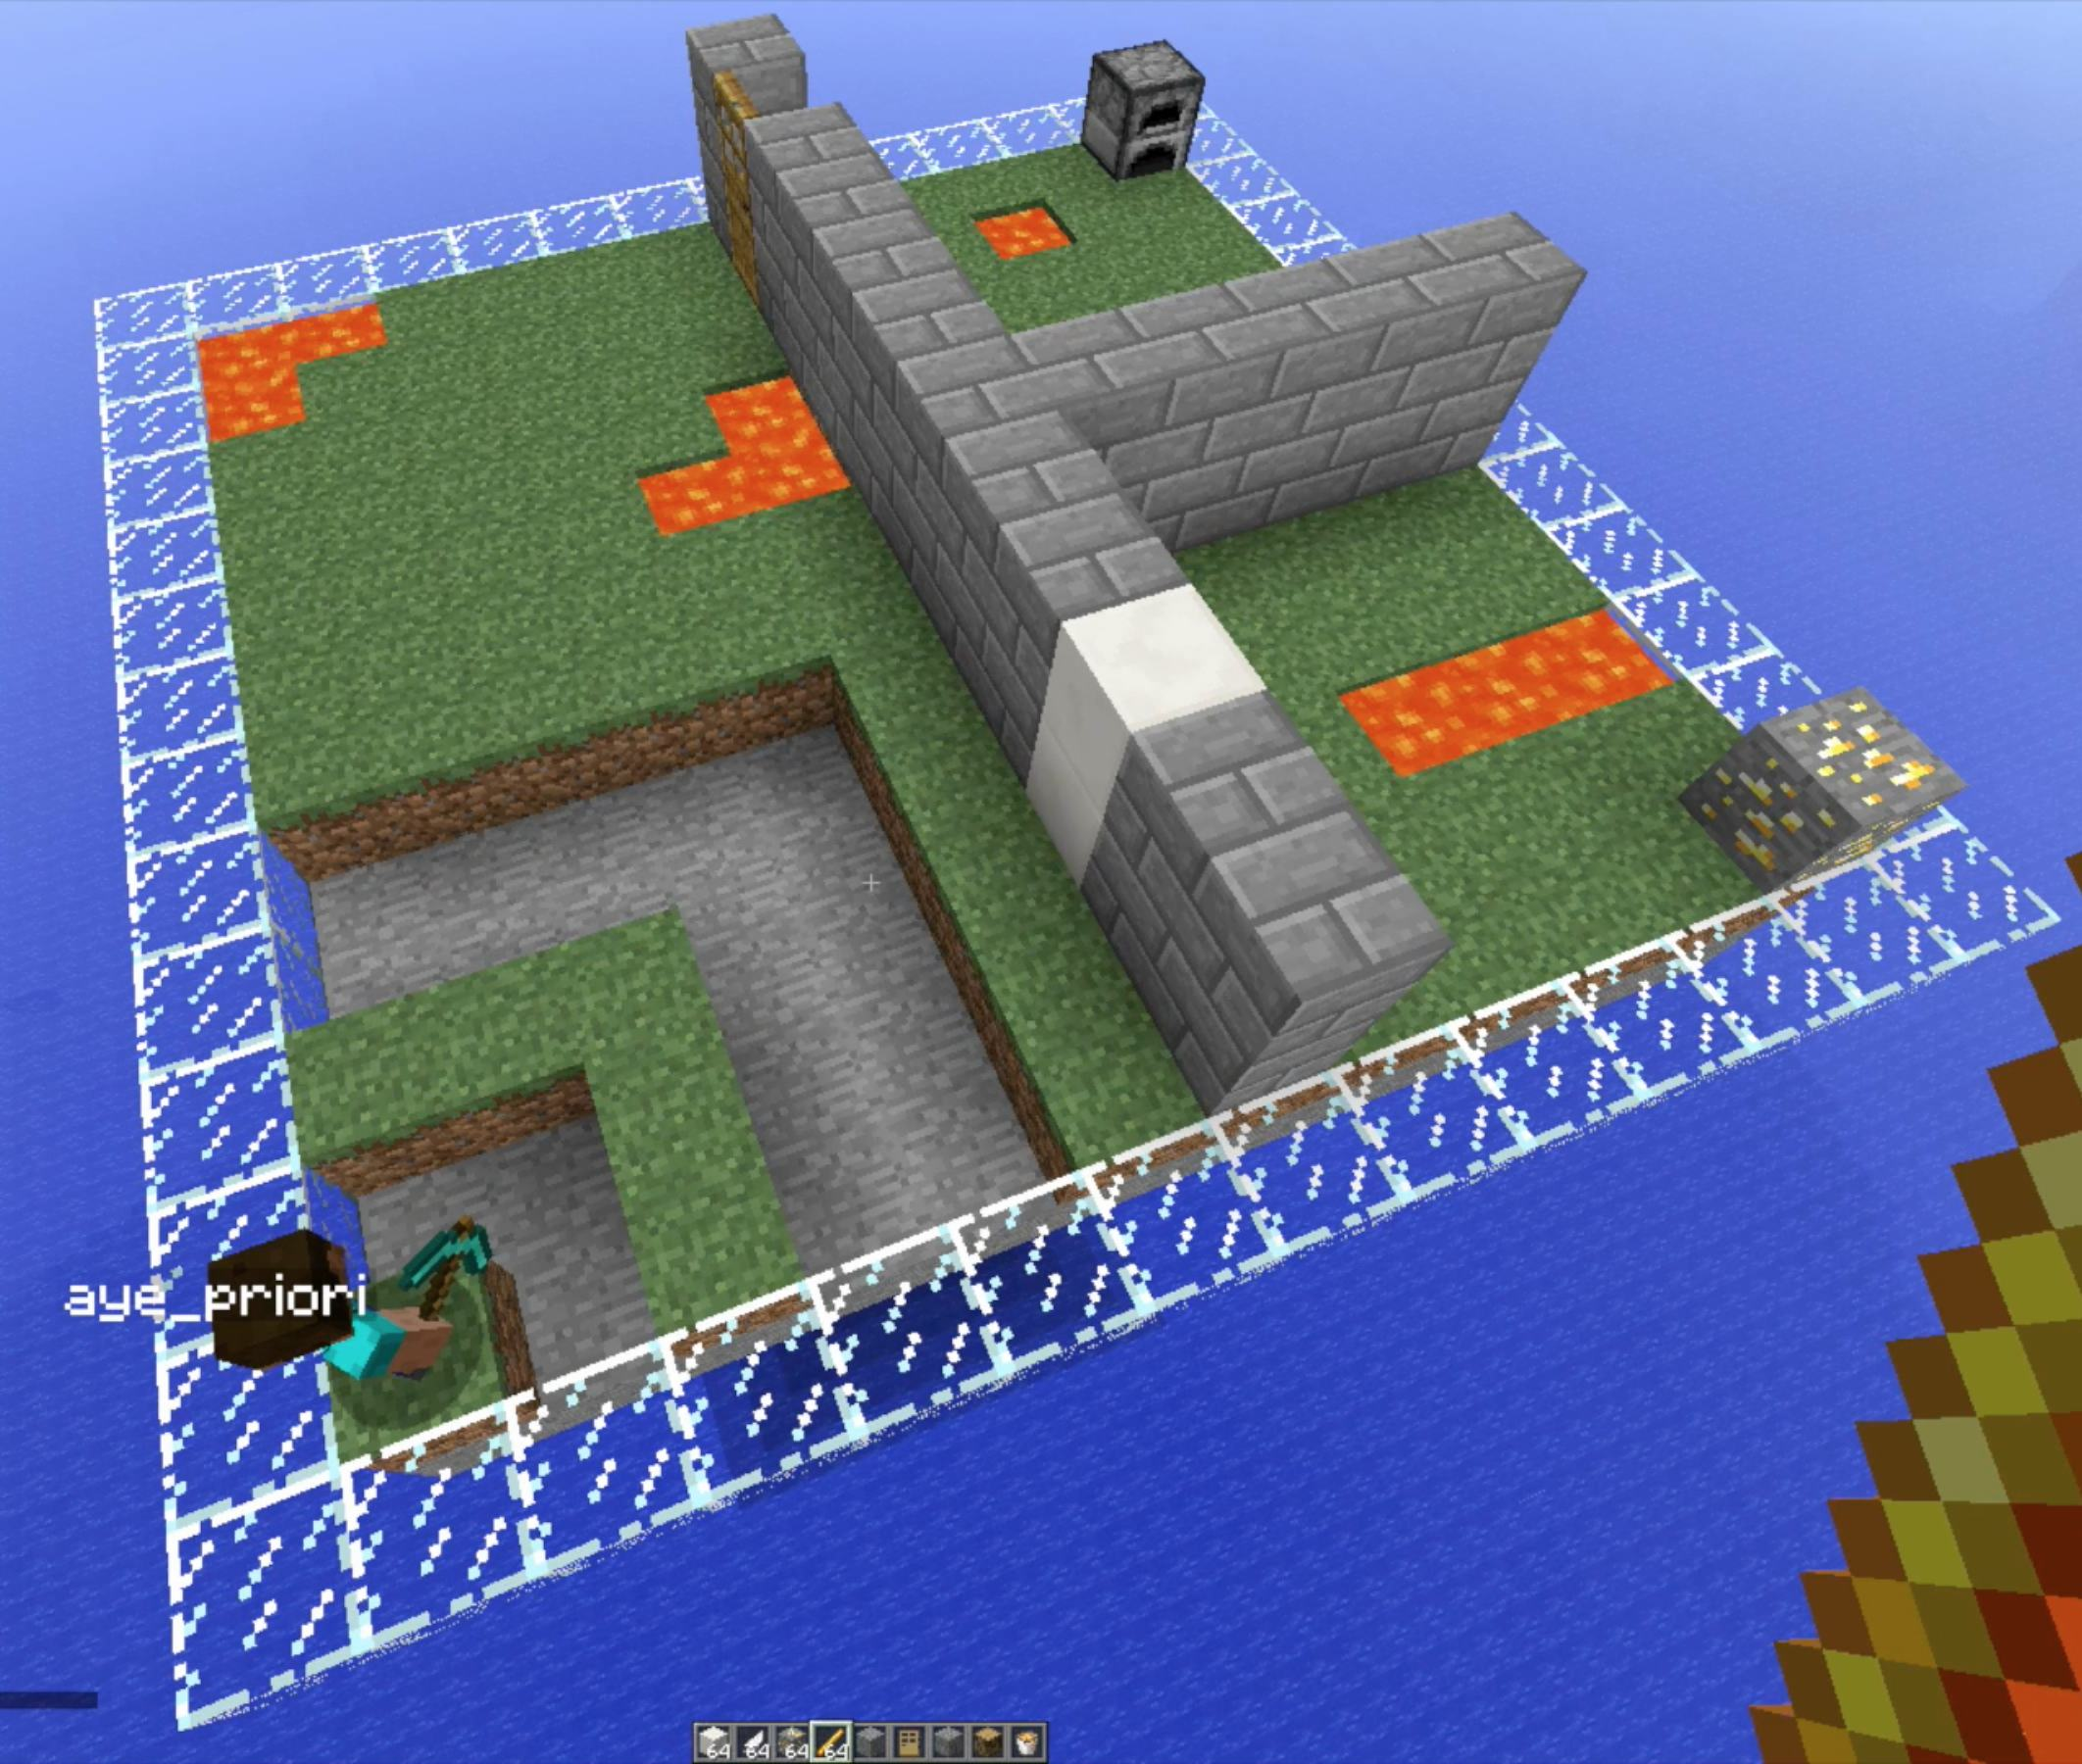
\includegraphics[scale=0.13]{figures/epicworld_1.jpg}%
  \caption{A gold smelting task in the Minecraft domain}
  \label{fig:minecraft}
\end{figure}

Our experiments consisted of 5 common tasks in Minecraft, including
constructing bridges over trenches, smelting gold, tunneling
through walls, basic path planning, and digging to find an object.  We tested on 
randomized worlds of varying size and difficulty. The generated test
worlds varied in size from tens of thousands of states to hundreds of thousands of states.

The training data consisted of 10 simple state spaces of each map type
(50 total), each map approximately a 1,000-10,000 state world with
randomized features that mirrored the agent's actual state space. All tests
conducted used the same training data.

The evaluation metric for each trial was the number of Bellman updates
that were executed by each planning algorithm, the accumulated reward,
and the CPU time taken to find a plan.  We terminated each planner
when the maximum change in the value function was less than 0.01 for
100 consecutive policy rollouts, or the planner failed to converge
after 1500 rollouts.  We set the reward function to $-1$ for all
transitions, except transitions to states in which the agent was on
lava, which returned $-10$. The goal was set to be terminal. The
discount factor was set to $\lambda = 0.99$. For all experiments,
movement actions (move, rotate, jump) had a small probability (0.05)
of incorrectly applying a different movement action.

\begin{table}[H]
\centering
\caption{RTDP vs. Learned Affordance-Aware RTDP}
\begin{tabular}{ c l  || c c c c}
  State Space	&	Planner 		&	CPU	&	Reward 	& Bellman \\ \hline
  Mine 	& 	\texttt{RTDP}  		& 	160.0s	&	-228.75	&	80610.7		\\
  		& 	\texttt{ARTDP}  	& 	{\bf 68.1s}	&	{\bf -12.4}	&	{\bf 16633.1}	\\  \hline
  Smelt	&	\texttt{RTDP}  		& 	639.4s	&	-231.4	&	99089.6		\\
  		&	\texttt{ARTDP}  	& 	{\bf 20.8s}	&	{\bf -11.9}	&	{\bf 4807.4}	\\  \hline
  Wall	&	\texttt{RTDP}  		& 	144.5s	&	-26.0		&	60994.9		\\
  		&	\texttt{ARTDP}  	& 	{\bf 116.6s}&	{\bf -17.9}	&	{\bf 23198}	\\  \hline
  Trench	&	\texttt{RTDP}  		& 	206.5s	&	{\bf -6.5}	&	19529.6		\\
  		&	\texttt{ARTDP}  	& 	{\bf 116.4s}&	-7.2		&	{\bf 10533.9}	\\ \hline
Plane	&	\texttt{RTDP}  		& 	1414.1s	&	{\bf -6.1}	&	30987		\\
  		&	\texttt{ARTDP}  	& 	{\bf 159.4s}&	{\bf -6.1}	&	{\bf 5096.2}	\\ 
\end{tabular}
\label{table:minecraft_results}
\end{table}

Table~\ref{table:minecraft_results} shows the average CPU time, accumulated reward, and Bellman updates 
for RTDP and affordance-aware RTDP (ARTDP) after planning in 20 different maps of each goal type (100 total). Because the planners were forced to terminate after only 1000 rollouts, they did not always converge to the optimal policy. 
As the results suggest, ARTDP found a better plan (-11.9 reward to -231.4 reward) in significantly less time than 
RTDP in the gold smelting task (6 seconds to 543 seconds), as well as the plane traversal task (17.5 seconds to 168.4 seconds).

\dnote{Put in a note about the threshold issues, maybe include the results below to reinforce threshold business}

%In some cases, ARTDP found a less optimal plan than RTDP - this is likely due to 
%the fact that the affordances pruned away actions that were optimal in some states. 
%If this were to happen consistently, the expert defined threshold could be lowered to 
%reduce the amount of pruning, raising the likelihood of finding the optimal policy. 
%Conversely, though, this reduces the speedups of affordance-aware planning. In 
%future work, we are considering an extension to our current sampling methods in 
%which the threshold iteratively becomes less conservative until an optimal policy is found.

%\begin{table}[H]
%\centering
%\begin{tabular}{ c l  || c c c c}
%  State Space	&	Planner 				&	CPU	&	Reward 	& Bellman \\ \hline
%  Mine 	& \texttt{RTDP}  			& 	129.1s	&	{\bf -33.55}	&	63291		\\
%  		& \texttt{ARTDP}  			& 	{\bf 65.6s}	&	-99.5		&	{\bf 16917}		\\  \hline
%  Smelt	&	\texttt{RTDP}  			& 	543.0s	&	-99.5		&	74260		\\
%  		&	\texttt{ARTDP}  		& 	{\bf 6.3s}	&	{\bf -6.3}	&	{\bf 1845}		\\  \hline
%  Wall	&	\texttt{RTDP}  			& 	55.4s		&	-8.6		&	29324		\\
%  		&	\texttt{ARTDP}  		& 	{\bf 14.8s}	&	{\bf -11.4}	&	{\bf 3955}		\\  \hline
%  Trench	&	\texttt{RTDP}  			& 	{\bf 30.2s}		&	{\bf -3.35}	&	{\bf 5070}		\\
%  		&	\texttt{ARTDP}  		& 	600.1s	&	-89.8		&	67625		\\ \hline
%Plane	&	\texttt{RTDP}  			& 	168.4s		&	-1.8		&	7954		\\
%  		&	\texttt{ARTDP}  		& 	{\bf 17.5s}	&	-1.8		&	{\bf 830}		\\ 
%\end{tabular}
%\caption{RTDP vs. Learned Affordance-Aware RTDP}
%\label{table:minecraft_results}
%\end{table}

% -- Subsection: Temporally Extended Actions --
\subsection{Temporally Extended Actions}
Additionally, we compared our approach to Temporally Extended Actions: 
macroactions and options. We compared RTDP with expert affordances, 
expert macroactions, and expert options, as well as the combination of 
affordances, macroactions, and options. We conducted these experiments 
with the same configurations as our Minecraft experiments. The option policies
and macroactions provided were hand coded by domain experts.

\dnote{New results incoming tomorrow}
% -- Figure: Temporally Extended Actions Results --
\begin{table}[H]
\centering
\caption{Affordances vs. Temporally Extended Actions}
\begin{tabular}{ l  || c c c c}
  Augmentation 					&	CPU	&	Reward 	& Bellman \\ \hline
  \texttt{RTDP}  					&		&	-1.05		&	1000		\\
  \texttt{w/ Opt}  				&		&	-1.05		&	1058		\\
  \texttt{w/ MA}  					&		&	-1.05		&	703.25		\\
  \texttt{w/ Affordances}  			& 		&	-1.05		&	204		\\
  \texttt{w/ Affordances+Opt}  		& 		&	-1.05		&	349.6		\\
   \texttt{w/ Affordances+MA}  		& 		&	-1.05		&	202.15		\\
   \texttt{w/ Affordances+MA+Opt}  	& 		&	-1.05		&	{\bf 180.9}		\\
\end{tabular}
\label{table:temp_ext_act_results}
\end{table}

\dnote{New results here incoming on 8/29}
Table~\ref{table:temp_ext_act_results} indicates the results of comparing RTDP
equipped with macro actions, options, and affordances across 10 different executions
in the same randomly generated Minecraft worlds. The planners were tasked with 
reaching a particular location, given a set of obstacles to overcome. As the results 
suggest, both macroactions and options add significant number of Bellman Updates to 
planning, and an increase in CPU time. This is due to the fact that the branching factor of the state-action space significantly increases when augmented with additional actions. Furthermore, computing the expected reward of applying an option is computationally expensive. With affordances, the planner completed in less CPU time, and with fewer 
bellman updates. This supports the claim that affordances can handle the augmented 
action space provided by temporally extended actions by pruning away unnecessary actions.

% -- Subsection: Learning Rate --
\subsection{Learning Rate}
Additionally, we conducted experiments in which we varied the number of states visited at training time. 
As in Table \ref{table:minecraft_results}, we randomly generated simple state spaces
containing several thousand states containing features that mirrored the agent's state
space at test time. We then solved the OO-MDP with knowledge bases learned from 
10 to 10000 states.\dnote{update when training complete}

\dnote{Experiments have not yet finished for learning rate (underway)}

% -- Figure: Learning rate results --
\begin{figure}[H]
\centering
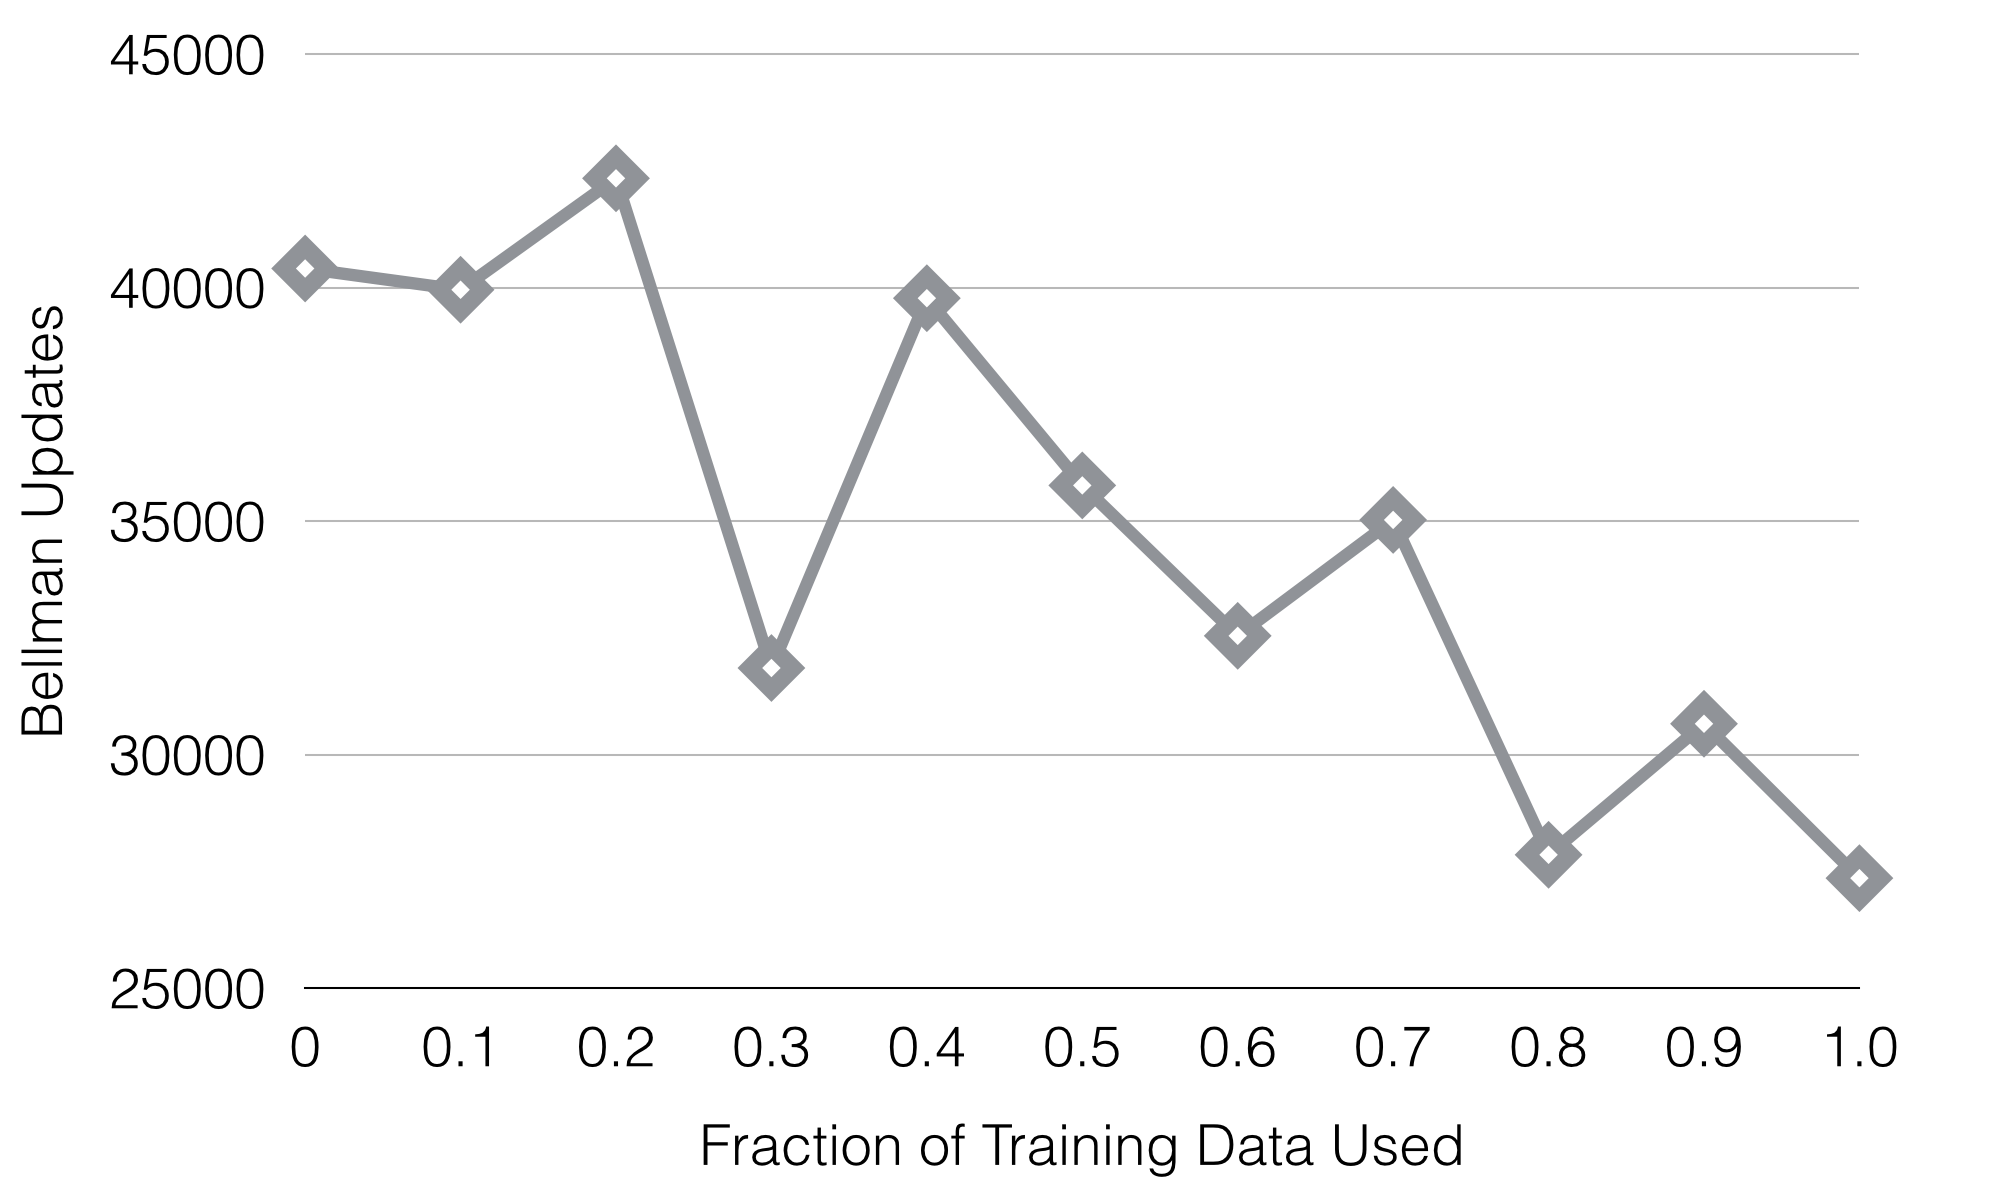
\includegraphics[scale=0.195]{figures/training_results.png}%
  \caption{PLACE HOLDER for learning rate results}
  \label{fig:training_results}
\end{figure}

% -- Subsection: Baxter --
\subsection{Baxter}

\dnote{Insert description of baxter stuff here}

\dnote{Experiments not yet finished}

% -- Figure: Baxter results/image
\begin{figure}[H]
\centering
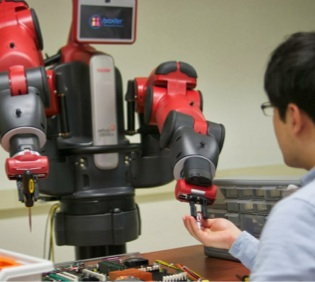
\includegraphics[scale=0.195]{figures/baxter_temp.jpg}%
  \caption{Placeholder for baxter results/image}
  \label{fig:baxter_results}
\end{figure}

% ====== Section: Related Work ======
\section{Related Work}
\label{sec:related-work}

In this section, we discuss the differences between
affordance-aware planning and other forms of knowledge engineering that
have been used to accelerate planning. We divide these approaches
into those that are built to plan in stochastic domains, and those that are
designed for use with deterministic domains.

% -- Subsection: Stochastic --
\subsection{Stochastic Approaches}

% --- Subsection: Temporally Extended Actions ---
\subsubsection{Temporally Extended Actions}
Temporally extended actions are actions that the agent can
select like any other action of the domain, except executing them
results in multiple primitive actions being executed in
succession. Two common forms of temporally extended actions are {\em
  macro-actions}~\cite{hauskrecht98} ~and {\em options}~\cite{sutton99}. 
Macro-actions are actions that always
execute the same sequence of primitive actions. Options are defined
with high-level policies that accomplish specific sub tasks. For
instance, when an agent is near a door, the agent can engage the
`door-opening-option-policy', which switches from the standard
high-level planner to running a policy that is hand crafted to open
doors. 

Although the classic options framework is not generalizable to different state spaces,
creating {\em portable} options is a topic of active research~\cite{konidaris07,konidaris2009efficient,Ravindran03analgebraic,croonenborghs2008learning,andre2002state,konidaris2012transfer}.

Given the potential for unhelpful temporally extended actions to negatively impact planning time~\cite{Jong:2008zr}, we believe combing affordances with temporally extended actions
may be especially valuable because it will restrict the set of temporally extended actions to those
useful for a task. We conducted a set of experiments to investigate this intuition. \dnote{Note about the results validating our hypotheses?}

% --- Subsection: Action Pruning ---
\subsubsection{Action Pruning}

Sherstov and Stone~\cite{sherstov2005improving} considered MDPs with a very large 
action set and for which the action set of the optimal policy of a source task could be 
transferred to a new, but similar, target task to reduce the learning time required to find
the optimal policy in the target task. The main difference between our affordance-based 
action set pruning and this action transfer work is that affordances prune away actions on 
a state by state basis, where as the learned action pruning is on per task level. Further, 
with lifted goal descriptions, affordances may be attached to subgoal planning for a significant
benefit in planning tasks where complete subgoal knowledge is known.

Rosman and Ramamoorthy~\cite{rosman2012good} provide a method for learning action
priors over a set of related tasks. Specifically, they compute a Dirichlet distribution over 
actions by extracting the frequency that each action was optimal in each state for each 
previously solved task.

There are a few limitations of the actions priors work that affordance-aware planning
does not possess: (1) the action priors can only be used with planning/learning algorithms
that work well with an $\epsilon$-greedy rollout policy; (2) the priors are only utilized for 
fraction $\epsilon$ of the time steps, which is typically quite small; and (3) as variance in
tasks explored increases, the priors will become more uniform. In contrast, affordance-aware
planning can be used in a wide range of planning algorithms, benefits from the pruned action
set in every time step, and the affordance defined lifted goal-description enables higher-level 
reasoning such as subgoal planning.

\dnote{Policy priors addition?}

% --- Subsubsection: Heuristics ---
\subsubsection{Heuristics}
Heuristics in MDPs are used to convey information about the value of a given state-action pair with respect to the task being solved and typically take the form of either {\em value function initialization},
or {\em reward shaping}. Initializing the value function to an admissible close approximation of the optimal value function has been shown to be effective for LAO* and RTDP~\cite{Hansen:1999qf}.

Reward shaping is an alternative approach to providing heuristics. The planning algorithm uses a modified version of the reward function that returns larger rewards for state-action pairs that are expected to be useful, but does not guarantee convergence to an optimal policy unless certain properties of the shaped reward are satisfied~\cite{potshap}.

A critical difference between heuristics and affordances is that heuristics are highly dependent on the reward function and state space of the task being solved, whereas affordances are state space independent and transferable between different reward functions. However, if a heuristic can be provided, the combination of heuristics and affordances may even more greatly accelerate planning algorithms than either approach alone.

% -- Subsection: Deterministic knowledge engineering approaches --
\subsection{Deterministic Approaches}

There have been several successful attempts at engineering knowledge to
decrease planning time for deterministic planners. These are fundamentally solving
a different problem from what we are interested in, but there approaches are interesting to consider.
\dnote{Need to rephrase this with justification for dealing with deterministic planners}.

% --- Subsubsection: Hierarchical Task Networks ---
\subsubsection{Hierarchical Task Networks}

\dnote{I think we should have a shoutout to Branavan's Learning High Level Plans from Text paper in this section (and include subgoal planning as part of this section}

\enote{I've been writing traditional as I expect we'll discover some HTNs that grapple with the issues stated below -- which we should probably cite}Traditional Hierarchical Task Networks (HTNs) employ \textit{task decompositions} to aid in planning. The goal at hand is decomposed into smaller tasks which are in turn decomposed into smaller tasks. This decomposition continues until primitive tasks that are immediately achievable are derived. The current state of the task decomposition, in turn, informs constraints which reduce the space over which the planner searches.

At a high level both HTNs and affordances fulfill the same role: both achieve action pruning by exploiting some form of supplied knowledge. HTNs do so with the use of information regarding both the task decomposition of the goal at hand and the sorts constraints that said decomposition imposes upon the planner. Similarly, affordances require knowledge as to how to extract values for propositional functions of interest by querying the state.

However there are three of essential distinctions between affordances and traditional HTNs. (1) HTNs deal exclusively with deterministic domains as opposed to the stochastic spaces with which affordances grapple. As a result they produce plans and not policies. (2) Moreover, HTNs do not incorporate reward into their planning. Consequently, they lack mathematical guarantees of optimal planning. \enote{I thinks We should double check this.} (3) On a qualitative level, the degree of supplied knowledge in HTNs surpasses that of affordances: whereas affordances simply require relevant propositional functions, HTNs require not only constraints for sub-tasks but a hierarchical framework of arbitrary complexity. Thus, despite a superficial similarity between affordances and HTNs wherein both employ supplied knowledge, the two deal with disparate forms of planning problems; HTN's planning problem is deterministic, reward-agnostic and necessitates a plethora of knowledge while affordances solve a planning problem that is stochastic, reward-aware and requires only relatively basic knowledge about the domain.
\enote{Need citations for HTNs}
\dnote{needs to be shorter}
% --- Subsubsection: Temporal Logic ---
\subsubsection{Temporal Logic}

Bacchus and Kabanza~\cite{Bacchus95usingtemporal,Bacchus99usingtemporal} provided
planners with domain dependent knowledge in the form of a first-order version of linear
temporal logic (LTL), which they used for control of a forward-chaining planner. With this methodology, 
a \textsc{Strips} style planner may be guided through the search space by checking 
whether candidate plans do not falsify a given knowledge base of LTL formulas, often
achieving polynomial time planning in exponential space.

The primary difference between this body of work and affordance-aware planning is that affordances may be learned (increasing autonomy of the agent), while LTL formulas are far too complicated to learn effectively, placing dependence on an expert.

% ====== Section: Conclusion ======
\section{Conclusion}
\label{sec:conclusion}
\dnote{Conclusion could use some work/rewriting}
We proposed a novel approach to representing transferable knowledge in terms of
{\em affordances}~\cite{gibson77} that allows an agent to efficiently prune actions 
based on learned knowledge, providing a significant reduction in the number of state-action
pairs the agent needs to evaluate in order to act near optimally. We demonstrated the 
effectiveness of the affordance model by comparing a RTDP to its affordance-aware
equivalent in a series of challenging planning tasks in the Minecraft domain. Further, we designed
a full learning process that allows an agent to autonomously learn useful affordances that may be used
across a variety of task types, reward functions, and state-spaces, allowing for convenient extensions 
to robotic applications.

We compared the effectiveness of augmenting planners with affordances compared to 
temporally extended actions. The results suggest that affordances, when combined with 
temporally extended actions, provide substantial reduction in the portion of the state-action 
space that needs to be explored.

Lastly, we deployed an affordance-aware planner on a robot in a collaborative cooking task with a massive 
state space. \dnote{Need to flesh out once we have more detail}.

In the future, we hope to automatically discover useful state-space-specific-subgoals online 
- a topic of some active research \cite{Mcgovern01automaticdiscovery,Simsek:2005:IUS:1102351.1102454}.
This will allow affordances to plug into high-level subgoal planning, which will reduce the size of the 
explored state-action space and improve the relevance of the action pruning. 

Additionally, we hope to explore additional methods that capitalize on the distribution over optimal actions, such as incorporating affordances with a forward search sparse sampling algorithm~\cite{walsh2010integrating}, or replacing the Naive Bayes model with a more sophisticated model, such as Logistic Regression or a Noisy-OR. We are also investigating methods of learning the thresholded value in a more principled way - one such approach is to initialize the planner with a strict threshold, and slowly relax the threshold until a near optimal policy is found. We are also interested in updating model parameters on-line by using planning data to update the distribution over optimal actions. 

Lastly, we hope to decrease the amount of knowledge given to the planner by learning predicates, or relations between predicates (i.e. Incremental Feature Dependency Discovery ~\cite{ICML2011Geramifard_473}) to further enhance autonomy.

{\small
\bibliographystyle{plainnat}
\bibliography{main}
}
\end{document}


